\documentclass[journal]{IEEEtran}

\usepackage[T1]{fontenc}
\usepackage{cite}
\usepackage{amsmath,amssymb}
\usepackage{graphicx}
\graphicspath{{figures/}}
\usepackage{booktabs}
\usepackage{multirow}
\usepackage{xcolor}
\usepackage{algorithm}
\usepackage{algpseudocode}
\usepackage{tikz}
\usetikzlibrary{positioning, arrows.meta}
\usepackage{hyperref}
\hypersetup{hidelinks}
\newcommand{\TODO}[1]{\textcolor{red}{[TODO: #1]}}

\begin{document}

\title{Two-Stage MQTT Gateway Security: Live Intrusion Filtering and Post-Quantum Re-Encryption on Raspberry Pi}

\author{Sheikh Sayed Bin Rahman, Kanita Jerin Tanha, Minsoo Kim, and Taesoo Jun%
\thanks{This research was funded by the National Research Foundation of Korea (NRF) grant funded by the Korea government (MSIT) (RS-2026-25497739, 34\%), the Innovative Human Resource Development for Local Intellectualization Program through IITP under MSIT (IITP-2026-RS-2020-II201612, 33\%), and the Basic Science Research Program through NRF under the Ministry of Education (2018R1A6A1A03024003, 33\%). \textit{(Corresponding author: Taesoo Jun.)}}%
\thanks{The authors are with the Pervasive Intelligent Computing Laboratory, Department of IT Convergence Engineering, Kumoh National Institute of Technology, Gumi, Republic of Korea (e-mail: sksayed@kumoh.ac.kr; kanitajerin17@kumoh.ac.kr; kms991022@kumoh.ac.kr; taesoo.jun@kumoh.ac.kr).}}

\markboth{IEEE Internet of Things Journal}%
{Rahman \MakeLowercase{\textit{et al.}}: Two-Stage MQTT Gateway Security}

\maketitle

\begin{abstract}
MQTT gateways face two threats at once: present-day network attacks that flood or probe the broker, and harvest-now-decrypt-later (HNDL) adversaries that record cloud-bound traffic for future quantum decryption. Recent work addresses these threats separately: intrusion detection systems are evaluated offline on datasets, while post-quantum cryptography (PQC) is benchmarked as isolated primitives, TLS handshakes, or hardware accelerators. We design, implement, and measure a two-stage gateway on Raspberry Pi hardware. Stage~1 intercepts MQTT-bound flows with Linux NetfilterQueue, extracts 32 flow features that can be reproduced from live packets, and classifies them with a LightGBM model trained on CICIoMT2024 and calibrated on local benign traffic (21 classes; 71.5\% offline accuracy, 0.709 macro-F1). Two policies turn its predictions into decisions: an attack prediction counts only if the client sent at least 30\% of the flow segment's payload bytes, and a connection is blocked only after two consecutive attack verdicts. Stage~2 re-encrypts messages that reach the gateway with ML-KEM-768, AES-256-GCM, and ML-DSA-65 (NIST Level~3 parameter sets) without device firmware changes. In the labelled two-Pi study the envelope is constructed on the gateway and is not transmitted; a separate three-Pi campaign forwards it over HTTPS to a LAN cloud receiver that verifies, decrypts, and rejects replays. In a labelled two-Pi testbed (five run types, four repetitions each, after separate development trials), Stage~1 flagged 1.0\% of benign verdicts in benign-only runs; with benign and attack traffic mixed, per-verdict precision was 0.999 and recall 0.994 (0.980 without UDP-flood verdicts; macro-averaged recall over the ten attack families 0.991), and every attack family was flagged in at least 91\% of its verdicts. The model's raw predictions on the same verdicts give a precision of only 0.930, because subscribers receive forwarded attack traffic. Detection is not the same as prevention: in IPS mode 80.6\% (R4) and 80.2\% (R5) of attack connections were blocked, and all benign messages reached Stage~2. Long-lived floods were always cut off. The unblocked remainder had been detected but received only one verdict: SYN-flood and leftover connect-flood attempts had typically already closed, so a block would not have cut a live socket, whereas all five slow-connection sockets stayed open on the broker until the attack window ended. Stage~1 needs a median 2.4~ms of processing per verdict and Stage~2 a median 2.1~ms of cryptographic work per message. Across ten KEM/signature configurations, ML-KEM pairings with ML-DSA or Falcon required 36--53\% less cryptographic time than ECDH+ECDSA for 5~KB payloads, while per-message key regeneration dominates handler latency for Falcon and SLH-DSA.
\end{abstract}

\begin{IEEEkeywords}
Edge computing, intrusion prevention, IoT gateway, LightGBM, ML-DSA, ML-KEM, MQTT security, post-quantum cryptography.
\end{IEEEkeywords}

% ═════════════════════════════════════════════════════════════════════════════
\section{Introduction}
\label{sec:intro}

\IEEEPARstart{M}{QTT}~\cite{mqtt_oasis} is the dominant publish--subscribe protocol for IoT telemetry. Its broker concentrates risk: a single gateway host receives traffic from many constrained devices and forwards it to cloud services. Two classes of adversary target this point. The first acts \emph{now}, flooding the broker with connections or publications, scanning it, or injecting malformed packets. The second acts \emph{later}: a harvest-now-decrypt-later (HNDL) adversary records cloud-bound traffic today and decrypts it once a cryptographically relevant quantum computer breaks the classical key exchange~\cite{shor1994,mosca2018}.

Recent work treats these adversaries separately. Machine-learning intrusion detection systems (IDS) for IoT report accuracies above 99\% on public datasets such as CICIoMT2024~\cite{ciciomt2024,abid2025gwo,wang2025skd,soomro2025roche}, but they are evaluated offline, are not placed in the packet path of a broker, and leave the payload exposed to HNDL collection. Post-quantum cryptography (PQC) studies benchmark the NIST standards ML-KEM~\cite{nist_fips203} and ML-DSA~\cite{nist_fips204} inside TLS~1.3 on a Raspberry Pi~\cite{shahid2026pqtls} or in dedicated ASIC hardware~\cite{dimatteo2026kem22}, but they assume an attack-free network path and do not address MQTT broker admission. None of the works we reviewed (Section~\ref{sec:related}) classifies live MQTT-bound traffic inline at the broker \emph{and} upgrades the received traffic to post-quantum protection, with both measured jointly on commodity gateway hardware.

This article closes that gap with a threat model, a full description of both stages, an offline and labelled live evaluation of the IDS/IPS, a ten-scheme PQC comparison, and a joint analysis of how the two stages compose. The primary labelled study covers the device-to-gateway path. A follow-on three-Pi campaign adds a second client address and a live HTTPS cloud receiver. The main contributions of this article are as follows.
\begin{enumerate}
  \item \textit{Two-Stage Gateway Design:} A Raspberry Pi gateway that classifies MQTT-bound TCP flows in the kernel packet path (NetfilterQueue + LightGBM, Stage~1) and re-encrypts messages that reach Stage~2 with ML-KEM-768 + AES-256-GCM + ML-DSA-65. The two-Pi study constructs the envelope on the gateway; the three-Pi study posts it over HTTPS to a cloud receiver that verifies the signature, decrypts, and rejects replays (Section~\ref{sec:design}).
  \item \textit{Offline and Labelled Live IDS/IPS Evaluation:} Per-class results on 484,255 held-out CICIoMT2024 flows with a feature set that is reproducible from live packets, and a labelled two-Pi evaluation (five run types, four repetitions each) that reports per-source flag rates, precision and recall, connection-level block rates by attack family, Stage~1 latency, attack packets admitted and dropped, and benign delivery with and without an infrastructure allow-list (Sections~\ref{sec:method}, \ref{sec:res-labelled}, \ref{sec:res-ids}, and~\ref{sec:res-e2e}).
  \item \textit{PQC Cost on the Gateway:} Per-operation re-encryption latency on 18,157 live messages and a ten-configuration comparison (seven PQC pairings, three classical baselines, three payload sizes, 18,000 messages), including the hidden cost of per-message key regeneration (Sections~\ref{sec:res-pqc} and~\ref{sec:res-matrix}).
  \item \textit{Composition and Deployment Lessons:} The live failure of a model that used all dataset features; the false positives of subscribers that receive forwarded attack traffic, removed by a client-share rule; the collateral blocking of long-lived benign connections and of the gateway's own subscriber, removed by a consecutive-verdict policy at the cost of leaving single-verdict attacks unblocked, including slow-connection sockets that remained open on the broker; and guidance on scheme choice, key caching, and bandwidth (Sections~\ref{sec:method}, \ref{sec:res-e2e}, and~\ref{sec:discussion}).
  \item \textit{Three-Pi and Cloud Evaluation:} Benign publishers on two client Pis, and attacks from a second address (alone or split with the first), under the same Stage~1 policies, with Stage~2 envelopes delivered to a LAN cloud receiver (Section~\ref{sec:res-three-pi}). One interrupted IPS repetition is excluded.
\end{enumerate}

The rest of this article is organized as follows. Section~\ref{sec:related} reviews related work. Section~\ref{sec:threat} states the threat model. Section~\ref{sec:design} describes the system, Section~\ref{sec:method} the evaluation methodology, and Section~\ref{sec:results} the results. Section~\ref{sec:discussion} discusses implications and limitations, and Section~\ref{sec:conclusion} concludes the article.

% ═════════════════════════════════════════════════════════════════════════════
\section{Related Work}
\label{sec:related}

\subsection{Machine-Learning Intrusion Detection for IoT}

Tree ensembles and lightweight deep models dominate recent IoT IDS work because flow features are low-dimensional and inference must be cheap~\cite{iot_ids_survey}. MQTTset~\cite{mqtt_ids_ml} established an MQTT-specific benchmark. CICIoMT2024~\cite{ciciomt2024} captures 18 attacks across MQTT, Wi-Fi, and Bluetooth in an IoMT testbed and reports offline baselines. Abid et al.~\cite{abid2025gwo} combine grey-wolf feature selection with a CNN-enhanced LightGBM and report near-perfect accuracy on CICIoT2023 and CICIoMT2024. Wang et al.~\cite{wang2025skd} compress an IDS with self-knowledge distillation and report over 99\% accuracy at reduced model size. Soomro et al.~\cite{soomro2025roche} train a federated IIoT IDS with homomorphic protection of model updates. All four evaluate on stored datasets with accuracy, F1, and confusion matrices; none is placed in the packet path of a live broker, reports per-flow verdict latency on gateway hardware, or protects the payload after admission.

\subsection{Post-Quantum Cryptography for IoT}

Surveys identify lattice-based schemes as the best fit for IoT~\cite{pqc_iot_survey}, and pqm4 showed that ML-KEM's predecessor runs in under a millisecond on Cortex-M4 microcontrollers~\cite{kyber_arm}. Malina et al.~\cite{malina2024mqttpqc} propose quantum-resistant MQTT communication. Shahid et al.~\cite{shahid2026pqtls} integrate ML-KEM and ML-DSA into TLS~1.3 with X.509 certificates on a Raspberry Pi~4 and report handshake latency and certificate overhead. Di~Matteo et al.~\cite{dimatteo2026kem22} build a unified ML-KEM accelerator on 22-nm ASIC and report area, power, and energy. These works measure primitives, handshakes, or silicon; they do not integrate with an IDS, do not upgrade legacy device traffic at the application layer, and evaluate a single scheme family.

\subsection{Positioning}

Table~\ref{tab:related} compares the six closest recent works with ours.

\begin{table*}[!t]
\centering
\caption{Comparison With Recent Related Work}
\label{tab:related}
\footnotesize
\begin{tabular}{p{2.8cm}p{2.0cm}p{1.6cm}p{2.8cm}p{2.2cm}p{4.0cm}}
\toprule
\textbf{Work} & \textbf{Live MQTT path} & \textbf{IDS/IPS} & \textbf{PQC} & \textbf{Hardware} & \textbf{Main metrics} \\
\midrule
Dadkhah et al.~\cite{ciciomt2024} & Dataset & Offline & -- & Testbed capture & Dataset, baselines \\
Abid et al.~\cite{abid2025gwo} & No & Offline & -- & Server & Acc., F1, ROC \\
Wang et al.~\cite{wang2025skd} & No & Offline & -- & Server & Acc., model size \\
Soomro et al.~\cite{soomro2025roche} & No & Federated & -- & Server & Acc., FL overhead \\
Shahid et al.~\cite{shahid2026pqtls} & TLS only & -- & ML-KEM/ML-DSA in TLS & Raspberry Pi 4 & Handshake, bytes \\
Di~Matteo et al.~\cite{dimatteo2026kem22} & No & -- & ML-KEM hardware & 22-nm ASIC & Area, power \\
\midrule
\textbf{This work} & \textbf{Yes} & \textbf{Inline IPS} & \textbf{10 configs; MQTT re-encrypt + HTTPS cloud} & \textbf{Raspberry Pi 4B + LAN receiver} & \textbf{FPR, block rate, delivery, verdict ms, crypto ms, cloud accept} \\
\bottomrule
\end{tabular}
\end{table*}

% ═════════════════════════════════════════════════════════════════════════════
\section{Threat Model and Design Goals}
\label{sec:threat}

\textit{System:} Constrained IoT devices publish to a broker on a gateway host; the gateway can forward admitted messages to a cloud receiver. The labelled two-Pi study measures the device-to-gateway path and gateway processing. The three-Pi study also measures HTTPS delivery to a cloud receiver on the same LAN, not a wide-area uplink. Devices are legacy: their firmware and device-side cryptography cannot be changed.

\textit{Adversaries:}
\begin{itemize}
  \item \textit{A1---Local network attacker:} Reaches the broker port and launches connection floods, publish floods, SYN/UDP/ICMP floods, scans, and malformed MQTT packets to exhaust or probe the broker.
  \item \textit{A2---HNDL observer:} Passively records gateway-to-cloud traffic and stores it until quantum key recovery becomes feasible.
  \item \textit{A3---Active uplink attacker:} Modifies, replays, or forges messages on the gateway-to-cloud link.
\end{itemize}
The gateway itself is trusted; compromise of the gateway host, side channels, and adversarial evasion of the classifier are out of scope and discussed in Section~\ref{sec:limits}.

\textit{Design Goals:}
\begin{itemize}
  \item \textit{G1:} Limit the broker resources consumed by A1 traffic by classifying flows inline and blocking client connections flagged as attacks.
  \item \textit{G2:} Give cloud-bound data confidentiality against A2 at NIST Level~3 (a design goal of the Stage~2 envelope, conditional on secure key generation and provisioning, Section~\ref{sec:keys}). The three-Pi study shows that a receiver can decapsulate and decrypt accepted envelopes; it is not an attack against a recorded uplink.
  \item \textit{G3:} Give cloud-bound data integrity and origin authentication against A3, and reject replays. The three-Pi receiver verifies the ML-DSA signature and rejects a sequence number older than the last accepted value for that device. It does not include an active forgery campaign.
  \item \textit{G4:} Require no device firmware changes.
  \item \textit{G5:} Keep per-message overhead small relative to typical publish intervals (seconds).
\end{itemize}

% ═════════════════════════════════════════════════════════════════════════════
\section{System Design}
\label{sec:design}

\subsection{Overview}

Fig.~\ref{fig:arch} shows the pipeline. All TCP and UDP traffic to and from the broker port enters a NetfilterQueue (NFQUEUE) handled by Stage~1. Packets reach the Mosquitto broker unless their client connection has already been blocked. Stage~2 subscribes to device topics, re-encrypts each message that it receives, and can post the envelope over HTTPS to a cloud receiver. In the two-Pi study the envelope is constructed and not transmitted; in the three-Pi study it is (Section~\ref{sec:keys}). A message reaches Stage~2 only if the gateway's subscriber remains connected, so Stage~1 admission to the broker is not the same as Stage~2 processing.

\begin{figure*}[!t]
\centering
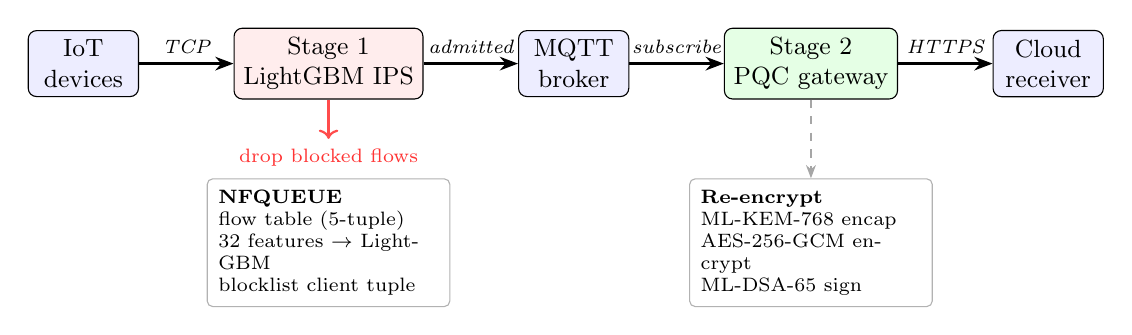
\begin{tikzpicture}[
    node distance=0.5cm and 0.4cm,
    box/.style={draw, rounded corners=3pt, fill=blue!7, minimum height=0.6cm, minimum width=1.4cm, font=\small, align=center},
    fwbox/.style={draw, rounded corners=3pt, fill=red!7, minimum height=0.6cm, font=\small, align=center},
    gwbox/.style={draw, rounded corners=3pt, fill=green!10, minimum height=0.6cm, font=\small, align=center},
    innerbox/.style={draw=gray!60, rounded corners=2pt, fill=white, font=\scriptsize, align=left, text width=2.8cm, inner sep=4pt},
    arr/.style={-Stealth, thick},
    darr/.style={-Stealth, dashed, gray!70},
    lbl/.style={font=\scriptsize\itshape, midway, above}
]
\node[box] (iot) {IoT\\devices};
\node[fwbox, right=1.2cm of iot, minimum width=2.0cm] (fw) {Stage 1\\LightGBM IPS};
\node[box, right=1.2cm of fw] (broker) {MQTT\\broker};
\node[gwbox, right=1.2cm of broker, minimum width=2.0cm] (gw) {Stage 2\\PQC gateway};
\node[box, right=1.2cm of gw] (cloud) {Cloud\\receiver};
\draw[arr] (iot) -- node[lbl]{TCP} (fw);
\draw[arr] (fw) -- node[lbl]{admitted} (broker);
\draw[arr] (broker) -- node[lbl]{subscribe} (gw);
\draw[arr] (gw) -- node[lbl]{HTTPS} (cloud);
\draw[->, red!70, thick] (fw.south) -- ++(0,-0.5) node[below, font=\scriptsize, red!80]{drop blocked flows};
\node[innerbox, below=1.0cm of fw] (fwd) {\textbf{NFQUEUE}\\flow table (5-tuple)\\32 features $\to$ LightGBM\\blocklist client tuple};
\node[innerbox, below=1.0cm of gw] (gwd) {\textbf{Re-encrypt}\\ML-KEM-768 encap\\AES-256-GCM encrypt\\ML-DSA-65 sign};
\draw[darr] (gw.south) -- (gwd.north);
\end{tikzpicture}
\caption{Two-stage gateway. Stage~1 classifies flows in the kernel packet path and blocks a client connection after two consecutive attack verdicts. Stage~2 builds an ML-KEM-768/ML-DSA-65 envelope. The two-Pi study stops at the gateway; the three-Pi study posts the envelope over HTTPS to a LAN cloud receiver.}
\label{fig:arch}
\end{figure*}

\subsection{Stage 1: LightGBM Flow Classifier and IPS}
\label{sec:stage1}

\textit{Interception:} An \texttt{iptables} rule sends packets for the broker port to NFQUEUE. A user-space callback parses IP/TCP (and UDP) headers with \texttt{dpkt}. To keep classification off the critical path, each packet is \emph{accepted back to the kernel before} the classifier runs; inference time therefore delays only later packets waiting in the queue, not the current one.

\textit{Flow State:} A bidirectional flow table keyed by the 5-tuple stores, for every packet, its frame length, IP TTL, TCP flags, header length, direction, and arrival time. A flow is classified 1)~when it terminates with FIN or RST after at least 3 packets; 2)~every 20 packets, so that long-lived connections such as MQTT sessions and publish floods receive one verdict per 20 packets; and 3)~by a background reaper when idle for 10~s. Flows that end or expire with fewer than 3 packets are logged as unclassified.

\textit{Features:} Each verdict uses 32 CICIoMT2024 features computed over the packets collected so far: packet rate (three columns); the share of packets carrying each TCP flag (FIN, SYN, RST, PSH, ACK, ECE, CWR); 15 protocol indicators (application protocol by port, transport, and link layer); and the minimum, maximum, mean, standard deviation, and total of the frame lengths, with the derived Magnitude and Radius. We matched each column to the semantics of the released data, which differ from their names in places: lengths include the 14-byte Ethernet header, and flag columns are shares rather than counts. The other 13 dataset columns are not used because a live flow cannot reproduce them. Eleven depend on how the dataset was windowed during capture (header length, flag counts, total sum, IAT, Number, Covariance, Variance, and Weight), and two mix packets from different flows (Duration, which tracks the IP TTL in the released data, and Protocol Type).

\textit{Classifier:} Features are standardized and passed to a 21-class LightGBM model~\cite{lightgbm2017} (benign plus 20 attack classes). The model predicts an attack when the arg-max class is not benign and the benign probability is below $1-\tau$, with $\tau = 0.5$.

\textit{Client-Share Rule:} The broker forwards every published payload to the subscribers of its topic, so the flow of a subscriber carries the attack traffic that it receives. An attack prediction is therefore kept only if the client sent at least a share $\gamma = 0.3$ of the segment's payload bytes (of its packets, if the segment carries no payload); otherwise the verdict is benign. Payload bytes are used rather than packets because a QoS~1 subscriber acknowledges every forwarded message and so sends about half of the packets but few of the bytes. The model's raw prediction is logged with every verdict.

\textit{Prevention:} In IPS mode, a client connection is blocked after $K = 2$ consecutive attack verdicts; a benign verdict resets the count. A block adds the client side of the flow (client IP, protocol, client port, broker port) to a blocklist; later packets matching it are dropped in the callback, and an \texttt{iptables} drop rule for the same tuple is inserted. Packets from the broker to a blocked connection are dropped as well and are no longer classified. Normalizing to the client side avoids blocking the broker's replies to other clients. Because the key includes the client port, a new connection from the same host is not covered by an earlier block. Blocks do not expire. Source addresses on an optional allow-list are exempt: their attack verdicts are logged but never blocked. In IDS mode, verdicts are logged and nothing is dropped.

\textit{Enforcement Timing:} Three intervals separate a flow's first packet from its first dropped packet: 1)~\emph{collection time}, until the flow has reached a classification trigger (minimum packet count with FIN/RST, every $N$ packets, or 10~s of idleness) for the $K$-th consecutive time; 2)~\emph{classification processing time}, for feature extraction, inference, and decision; and 3)~\emph{enforcement delay}, from the blocking verdict to the next packet of the blocked tuple. Every packet before the blocking verdict is admitted to the broker. Stage~1 therefore cuts off the remainder of long-lived attack connections, such as publish floods, but cannot stop connections that finish before a second verdict: flows shorter than the minimum packet count are never classified, and a connection that receives only one verdict, such as a SYN-flood or connect-flood attempt classified on FIN/RST or a slow connection classified once when idle, is detected but never blocked. For connections that have already ended, a block would cover only a finished tuple.

\subsection{Stage 2: Post-Quantum Re-Encryption}
\label{sec:stage2}

For every message received on a device topic, Stage~2 executes Algorithm~\ref{alg:reenc}. If the device used an encrypted scheme, the gateway first recovers the plaintext with the device key. It then encapsulates a fresh ML-KEM-768 shared secret to the cloud public key, encrypts the plaintext with AES-256-GCM under that secret and a random 96-bit nonce, and signs the encoded envelope with the gateway's ML-DSA-65 key.

\begin{algorithm}[!t]
\caption{Stage 2 Re-Encryption of a Message $m$ Received by Stage 2}
\label{alg:reenc}
\begin{algorithmic}[1]
\State $p \gets \textsc{DeviceDecrypt}(m)$ \Comment{identity if plaintext}
\State $(c_\mathrm{kem}, ss) \gets \textsc{ML-KEM-768.Encaps}(pk_\mathrm{cloud})$
\State $\eta \xleftarrow{\$} \{0,1\}^{96}$
\State $c_\mathrm{aes} \gets \textsc{AES-256-GCM}_{ss}(p, \eta)$
\State $M \gets \textsc{Encode}(id, seq, c_\mathrm{kem}, \eta, c_\mathrm{aes})$
\State $\sigma \gets \textsc{ML-DSA-65.Sign}(sk_\mathrm{gw}, M)$
\State \textbf{return} $\{id, seq, c_\mathrm{kem}, \eta, c_\mathrm{aes}, \sigma\}$ \Comment{envelope for the cloud}
\end{algorithmic}
\end{algorithm}

\textit{Signed Encoding:} $\textsc{Encode}$ outputs a fixed domain tag followed by the five fields $id$ (UTF-8), $seq$ (unsigned 64-bit, big-endian), $c_\mathrm{kem}$, $\eta$, and $c_\mathrm{aes}$, each prefixed by its 4-byte big-endian length. Length prefixes make the encoding unambiguous: two different field tuples can never produce the same signed bytes. The Stage~2 timings in Section~\ref{sec:res-pqc} were recorded with this encoding.

\textit{Security Properties:} By construction, a fresh encapsulation per message gives each message an independent key, so compromise of one message key does not expose others, and the IND-CCA2 security of ML-KEM-768 protects the uplink against A2 at NIST Level~3. ML-DSA-65 (EUF-CMA) over the encoded envelope gives integrity and gateway origin authentication against A3, and binding the signature to $(id, seq)$ allows a cloud receiver that tracks the last accepted $seq$ per device to reject replays. Signing the ciphertext rather than the plaintext also prevents an observer from confirming guesses of low-entropy sensor readings against a public signature. Cloud-side signature verification, decryption, and replay rejection are protocol properties of the receiver. The three-Pi study runs that receiver on the LAN (Section~\ref{sec:res-three-pi}). These properties hold for a deployment only if keys are generated with a cryptographically secure random-number generator and the cloud public key and gateway verification key are provisioned authentically. Device-to-gateway keys in both studies still come from the deterministic shared secret of Section~\ref{sec:keys}; the cloud KEM key and the gateway signing key used on the HTTPS path are generated separately, and each private key stays on the machine that created it. The device-to-gateway link keeps whatever scheme the device already uses (AES-256 under Grover retains 128-bit security), which meets G4 but does not add forward secrecy on that segment.

\subsection{Key Provisioning and Experimental Assumptions}
\label{sec:keys}

\textit{Provisioning:} Before the experiments, a single 256-bit master secret, written as 64 hexadecimal characters, is placed out of band in a local environment file on the experimental nodes. Each process loads it at start-up; it is never sent over MQTT or any other network channel.

\textit{Derivation:} Every key is derived from the master secret with HKDF-SHA256~\cite{rfc5869} (no salt) under a domain-separated context string that names the algorithm and, where applicable, the device, e.g., \texttt{aes:}$\langle id\rangle$, \texttt{ecdsa-p256:}$\langle id\rangle$, \texttt{kem:}$\langle alg\rangle$\texttt{:keypair}, and \texttt{sig:}$\langle alg\rangle$\texttt{:}$\langle id\rangle$\texttt{:keypair}. AES-256 and ChaCha20-Poly1305 keys are taken directly from HKDF output, and P-256 private keys are HKDF output reduced modulo the group order. PQC key pairs are produced by the standard liboqs key-generation routines while the liboqs random-number source is temporarily replaced, through its custom-RNG interface (\texttt{OQS\_randombytes\_custom\_algorithm}), by a callback that returns a deterministic, non-repeating stream: SHAKE-256 in counter mode, keyed by a 64-byte HKDF output. After key generation, including on error, the system RNG is restored (\texttt{OQS\_randombytes\_switch\_algorithm}). Because the liboqs RNG is process-wide, a lock serializes key generation, encapsulation, and signing, so that no other liboqs call in the process draws from the callback while it is installed. The construction serves experimental reproducibility only: anyone who holds the master secret can regenerate every key (see below). The live evaluation (Section~\ref{sec:protocol}) ran with this construction. The development sessions and the scheme comparison (Section~\ref{sec:res-matrix}) ran with an earlier callback that repeated the 64-byte HKDF output cyclically, which is not a cryptographically secure generator; that change affects how keys are generated, not the operations timed on keys in memory, but it does fall inside the handler time of the scheme comparison, where PQC key pairs are regenerated per message. The hook requires the bindings to use the same liboqs shared library; all real-liboqs PQC messages in the scheme comparison were accepted, which requires matching key pairs on client and gateway. Every node therefore reproduces the same key pairs without a key exchange. KEM key pairs are scoped per algorithm, so all devices encrypt to one gateway KEM key per algorithm; signature key pairs are scoped per device. Encapsulation randomness and AES-GCM nonces come from the system RNG.

\textit{Purpose and Measurement:} This setup makes runs reproducible and keeps key distribution out of the measured path: provisioning happens before any measurement and is not part of any reported latency. The scheme-comparison gateway is stateless and rederives the gateway KEM key pair and the sending device's verification key for every message. This regeneration falls inside the total handler time but outside the decapsulation, decryption, and verification timers, and Section~\ref{sec:res-matrix} reports the resulting non-cryptographic time separately. Stage~2 likewise derives its keys inside the handler, before its encapsulation timer starts.

\textit{Cloud Receiver:} Two configurations are used. In the two-Pi study (R1--R5), Stage~2 constructs the envelope and does not transmit it; those sessions measure gateway-side encapsulation, encryption, and signing only. In the three-Pi study, a background thread posts each envelope over HTTPS to a receiver on the same Wi-Fi LAN. The MQTT callback does not wait for the HTTP response, so HTTPS time is not added to the Stage~2 CSV. The receiver holds its own ML-KEM-768 private key, checks the gateway's ML-DSA-65 signature against a pinned public key, decapsulates, decrypts with AES-256-GCM, and accepts a message only if its sequence number is strictly newer than the last accepted value for that device identifier. An equal sequence number is a duplicate retry; an older one is a replay and is rejected. The receiver is a LAN stand-in, not a wide-area cloud, and the uplink is not subjected to an active forgery or HNDL experiment.

\textit{Trust Assumptions:} The experiments assume a single trusted administrative domain. In the two-Pi sessions, the broker, both stages, and the gateway's own subscriber run on one Raspberry Pi, and the benign clients and attack generators run on a second Raspberry Pi on the same Wi-Fi network. In the three-Pi sessions a third Raspberry Pi is a second client, and a PC on the same LAN is the cloud receiver. All nodes are controlled by the researchers. The master secret is assumed to be unavailable to attackers; the attack generators do not use it or any derived key. The secret is not rotated during the reported experiments. These are experimental assumptions, not security guarantees.

\textit{Limits of a Shared Secret:} A shared master secret is a single point of failure: whoever obtains it can derive every key derived from it, including device keys and, in the two-Pi study, the gateway KEM private key derived from that secret. The three-Pi HTTPS path uses a separate cloud KEM private key that the gateway does not hold. Deterministic shared-seed key generation is a controlled-testbed convenience, not a recommended production provisioning method. The NIST levels quoted in this article therefore describe the evaluated parameter sets, not the experimental key material: the experiments measure performance and do not establish production-grade post-quantum security. A production deployment requires independently provisioned device keys, private keys protected in hardware (e.g., a secure element or TPM), separate cloud key management in which the gateway never holds the cloud private key, and key rotation and revocation. The reported encapsulation, decapsulation, signing, and verification times measure operations on keys already in memory and do not depend on how those keys were generated. Production key management (enrolment, certificate validation, hardware key access, rotation, and revocation) would add overhead that we do not measure.

\subsection{Implementation}

Both stages run on a Raspberry Pi~4B (BCM2711, four Cortex-A72 cores at 1.8~GHz, 4~GB LPDDR4) under Python~3.11. In the two-Pi sessions, benign clients and attack generators run on a second Raspberry Pi~4B. In the three-Pi sessions, a third Raspberry Pi~4B is a second client, and a PC on the same LAN runs the HTTPS receiver. All nodes join the same Wi-Fi access point (a mobile hotspot). Stage~1 uses \texttt{NetfilterQueue}, \texttt{dpkt}, and LightGBM; Stage~2 uses \texttt{liboqs-python}~\cite{oqs2023}, the \texttt{cryptography} package for AES-GCM, and Paho-MQTT with Mosquitto. Timestamps come from \texttt{time.perf\_counter\_ns()}, and records are written by a background thread to avoid perturbing measurements.

% ═════════════════════════════════════════════════════════════════════════════
\section{Evaluation Methodology}
\label{sec:method}

\subsection{Model Training and Calibration}
\label{sec:training}

\textit{Data and Split:} The model uses the CICIoMT2024 Wi-Fi/MQTT flow rows of the dataset's released test partition (1,614,182 rows, 21 classes); the released training partition is not used. A stratified, row-level 70/30 split with a fixed seed gives 1,129,927 training and 484,255 test rows. Because the split is by row rather than by capture, rows from the same capture can fall on both sides: the test split is held out from training but is not independent of the training captures.

\textit{Training:} The 32 features of Section~\ref{sec:stage1} are standardized with statistics fitted on the training split, and a multiclass LightGBM model (learning rate 0.05, 31 leaves, at most 100 rounds) is trained with early stopping on a stratified 10\% validation split carved from the training split. The test split is used only for the final metrics: per-class precision, recall, F1, accuracy, and macro-F1. The hyperparameters are fixed values carried over from an earlier notebook; no search was run in this work. The 13 excluded columns were chosen by whether the live extractor can reproduce them, not by test performance. Training took 14.0~s.

\textit{Pilot and Calibration:} A pilot benign-only session (C1, 10.6~min) on the live testbed, run with an earlier model that used all 45 dataset features, showed severe dataset shift. That model labelled 96.4\% of the verdicts on benign client connections (242 of 251) and all 125 verdicts on the gateway's own subscriber as attacks. We then made two changes together. First, the model was restricted to the reproducible features. Second, the 375 benign flow segments of C1 (250 from the client-Pi benign clients and 125 from the gateway subscriber), rebuilt from its packet log with the live classification triggers, were each replicated 20 times (7,500 rows) and appended to the training split after the train/test split. They therefore enter the scaler fit and the early-stopping validation split, but never the test split. The model was trained once, and the offline metrics reported in Section~\ref{sec:res-offline} are those of this calibrated model; an uncalibrated 32-feature model was not evaluated. The model was not changed afterwards; the Stage~1 decision policies and attack rates were set later on development sessions (Section~\ref{sec:protocol}). C1 is not used in any reported live result. However, C1 used the same benign generators, with identical parameters, and the same gateway subscriber as the evaluation, so the live false-positive rates describe a system calibrated on similar local benign traffic. Because both changes were introduced together, the reduction from 96.4\% in C1 to the 1.0--1.7\% of benign-only sessions cannot be attributed to either change alone.

\subsection{Live Workloads}

\textit{Benign Clients:} Four generators model legitimate devices: a \emph{steady} sensor publishing every 2~s; a \emph{mixed} device with random 1--3~s intervals and occasional idle periods; a \emph{burst} device that sends 3--8 messages at 5~msg/s and then idles for 5--15~s; and a monitoring \emph{subscriber} to all device topics (QoS~1). Each publisher embeds a device identifier and a monotonic sequence number in every message and logs every publish with its result code. Stage~2's own subscriber runs on the gateway host and is treated as infrastructure.

\textit{Attack Clients:} Ten generators reproduce CICIoMT2024 MQTT and TCP/IP attack families against the broker port: MQTT publish flood, malformed MQTT packets, slow-connection (Slowloris-style) exhaustion holding 5 connections, MQTT connect flood (serial and with 5 parallel threads), port scan (ports 1870--1900), vulnerability scan, UDP flood (1 and 5 threads), and TCP SYN flood. The publish flood sends 40 messages/s, about 80 packets/s in both directions, within the 74--90 packets/s median rate of the dataset's publish-flood classes. The UDP floods send 500 datagrams/s in total (one thread, or five at 100/s) with 8-byte payloads, which reproduces the 50-byte frames of the dataset's UDP classes but stays well below their median rates of about 21,000--27,000 packets/s, which the Python NFQUEUE path on the gateway cannot absorb. All other generators send one message, connection, or packet per second per thread. ICMP floods and MQTT replay are outside the evaluated live scope, although ICMP floods belong to A1 (Section~\ref{sec:threat}). ICMP carries no port and does not match the broker-port NFQUEUE rules, and the replay generator requires a recorded benign capture, which was not available.

\subsection{Live Testbed, Runs, and Metrics}
\label{sec:protocol}

\textit{Testbed:} The gateway Pi runs Stage~1, the Mosquitto broker, and Stage~2; a second Pi runs all benign clients and attack generators, so live traffic crosses a Wi-Fi link. A control agent on the gateway starts every session from a clean state (broker restarted, block rules cleared) with identical Stage~1 settings (Section~\ref{sec:stage1}, threshold $\tau = 0.5$), and a runner on the client Pi then starts the workload.

\textit{Development Trials:} The Stage~1 policies and the attack rates were set on development sessions that are not part of the reported results. Three repetitions of the five run types below, with blocking after a single attack verdict, no client-share rule, and every attack at one event per second, showed three problems: the monitoring subscriber was flagged in 43\% of its verdicts when attacks ran, single false verdicts blocked 8--13 benign connections per IPS session, and the UDP and publish floods were almost never flagged. Replaying the logged packets offline through the deployed model and the live classification triggers, we chose $\gamma$ and $K$ on the first repetition and checked them on the other two, and found that the missed floods ran far below the rates, and for UDP used far larger frames, than their dataset classes. Two single-repetition trials followed. The first used a packet-count share, which failed because the QoS~1 subscriber acknowledges every forwarded message; it led to the byte share and to dropping the broker's packets to blocked connections, whose leftover segments were otherwise reclassified. The second confirmed the final configuration. The reported sessions then ran on a single code revision, with no setting changed between them. The development sessions used the same testbed, benign generators, and gateway subscriber as the evaluation, so the policies were tuned on traffic similar to the evaluation traffic.

\textit{Runs:} Five run types are each repeated four times (20 sessions), and we report the mean $\pm$ standard deviation over repetitions. A fifth repetition was interrupted by a Wi-Fi outage and is excluded entirely.
\begin{itemize}
  \item \textit{R1:} Benign clients only for 10~min, IDS mode.
  \item \textit{R2:} The ten attacks in sequence, each for 60~s with 20~s gaps, without benign clients, IDS mode.
  \item \textit{R3:} The R2 attack sequence with benign clients running throughout, IDS mode.
  \item \textit{R4:} As R3 in IPS mode, with the loopback address allow-listed so that the gateway's own subscriber cannot be blocked.
  \item \textit{R5:} As R4 without the allow-list.
\end{itemize}
R2--R5 sessions last 14.2~min each.

\textit{Three-Pi Runs:} After the two-Pi study, five further run types (E1--E5) were each repeated three times on three Raspberry Pis plus the LAN cloud receiver. Pi~A is the session controller. Pi~B joins every session: benign publishers on E1, the full attack list on E2 and E3, and the odd-indexed half of that list on E4 and E5. Pi~A runs the even-indexed half on E4 and E5, so the two halves are disjoint and together match one full attack pass. E1, E3, and E5 use IPS with the loopback allow-list; E1 and E3 also exempt the benign controller address, and E1 exempts Pi~B once it registers, because both of its roles are benign. E2 and E4 are IDS only. One E3 repetition stopped early (14 of 184 benign publishes reached Stage~2, and only two attack connections were labelled) and is excluded; E3 below is the mean of the other two. On E2 and E3, Pi~A keeps the session open long enough for Pi~B to finish all ten attacks (about 14.7~min in each retained E2 repetition).

\textit{Ground Truth:} The client Pi logs the local port of every benign connection, the start and end of every attack window, and every benign publish; the clock offset between the Pis is measured at session start (at most 5.6~ms). Each flow seen by Stage~1 is labelled from these logs: flows from the loopback or gateway address are \emph{infrastructure}; flows from the client Pi on a logged benign port are \emph{benign}, attributed to their client; and other client-Pi flows are attributed to the attack whose window, extended by the flow timeout plus 5~s, contains the first packet of the classified flow segment. Every classified client-Pi flow of the reported sessions received a label.

\textit{Metrics:} Detection is reported per classification verdict, not per independent connection. A long-lived connection receives one verdict per 20 packets, and a connect-flood connection one or two, so each source contributes in proportion to its verdicts. The \emph{flag rate} of a source is the share of its verdicts that are attacks; precision, recall, F1, and accuracy are computed over attack and benign-client verdicts, with infrastructure reported separately. Each classified flow segment starts afresh, because the flow entry is reset after every verdict. In IDS sessions, the UDP floods produce about 2,880 of the roughly 4,120 attack verdicts, so we also report recall without UDP-flood verdicts, the flag rate of every attack family, and a \emph{macro-averaged attack-family recall}: the unweighted mean of the ten families' flag rates, computed per session and then averaged over repetitions. Each workload counts equally, whether it produces 1 verdict or 1,400.

For IPS runs, detection and blocking are reported separately. An attack connection is \emph{detected} if it received at least one attack verdict, and \emph{blocked} if a block event was recorded for its client tuple. The \emph{block rate} is blocked connections divided by labelled attack connections of that family (or of all families). The \emph{benign delivery ratio} is the share of benign publish calls that returned success at the client library whose (device, sequence number) reached Stage~2. Success here means return code 0, i.e., the message was queued for sending, not acknowledged. \emph{Packets before block} counts, for each blocked attack connection, the packets in both directions of its classified segments up to and including the segment whose verdict triggered the block; it is averaged over blocked attack connections only. \emph{Attack packets dropped} sums the \texttt{iptables} block-rule counters and in-callback drops of client packets for tuples whose blocked connection is labelled as an attack. The two counts are disjoint: block rules are inserted ahead of the NFQUEUE rules, so a packet that matches a rule never reaches the callback. Dropped broker packets to blocked connections, and drops on blocked benign and infrastructure connections, are reported separately, and blocked connections are counted from block events.

\subsection{PQC Measurements}

\textit{Stage~2 on Live Traffic:} We time KEM encapsulation, AES-GCM encryption, signing, their sum, and the full handler (MQTT callback to completion) for every message received by the gateway subscriber in R1 and R3--R5. These timers are gateway-side processing costs; they are not added to Stage~1 classification time to form an end-to-end latency, and they do not include broker transit or cloud delivery. The live benign clients publish unencrypted JSON, so $\textsc{DeviceDecrypt}$ is the identity and these messages carry no device-side PQC; Stage~2 alone applies post-quantum protection, at the gateway. The constructed envelope is logged and not forwarded.

\textit{Scheme Comparison:} This separate benchmark evaluates device-to-gateway PQC: clients encrypt padded payloads of 5,120, 10,240, and 102,400 bytes under ten configurations (Table~\ref{tab:matrix}), 600 messages per configuration and size (18,000 messages, all accepted), and the gateway times decapsulation, decryption, and verification. Security level $L$ is the minimum NIST level of the KEM and signature. The configurations were measured sequentially in one session each, without interleaving or repeated sessions. PQC operations use liboqs; P-256 ECDH and ECDSA use OpenSSL through Python's \texttt{cryptography} package. AES-256-GCM and ChaCha20-Poly1305 are symmetric-only reference configurations: they perform no public-key establishment or signature verification and are not security-equivalent alternatives to the asymmetric configurations.

\textit{Timer Boundaries:} The crypto timer is the sum of the key-establishment, decryption, and verification timers; Base64 decoding, JSON handling, and logging fall outside it but inside the total handler time. The timers are not perfectly equivalent across libraries: the ECDH timer includes parsing the ephemeral public point and the HKDF derivation of the AES key, whereas the PQC decapsulation timer covers liboqs decapsulation without equivalent Base64 parsing or a KDF. The ECDH+ECDSA handler caches its static ECDH key and the device verification keys, whereas the PQC handler regenerates its key pairs for every message outside the crypto timer.

% ═════════════════════════════════════════════════════════════════════════════
\section{Results}
\label{sec:results}

\subsection{Offline Classifier Performance}
\label{sec:res-offline}

On the held-out set the model reaches 71.5\% accuracy, 0.709 macro-F1, and 0.706 weighted F1 (Fig.~\ref{fig:offline}). Restricting the model to live-reproducible features costs offline accuracy: the earlier 45-feature model reached 97.85\% accuracy and 0.900 macro-F1 on a held-out set of the same size but failed on live traffic (Section~\ref{sec:training}). Benign traffic is still recognized with 0.955 precision and 0.972 recall, so 2.8\% of benign test flows are assigned to an attack class. SYN floods (F1 0.96--0.98), MQTT connect floods (0.88--0.99), port scans (0.947), and TCP DDoS (0.903) remain well separated, and publish floods reach 0.83--0.85 and malformed MQTT 0.719. The loss concentrates in classes that the excluded windowing and timing columns used to separate: UDP floods (0.30--0.64), ICMP floods (0.55--0.68), TCP DoS (0.705), and low-volume reconnaissance such as OS scan (0.656), vulnerability scan (0.306), and ping sweep (0.216, only 56 test flows).

\begin{figure}[!t]
\centering
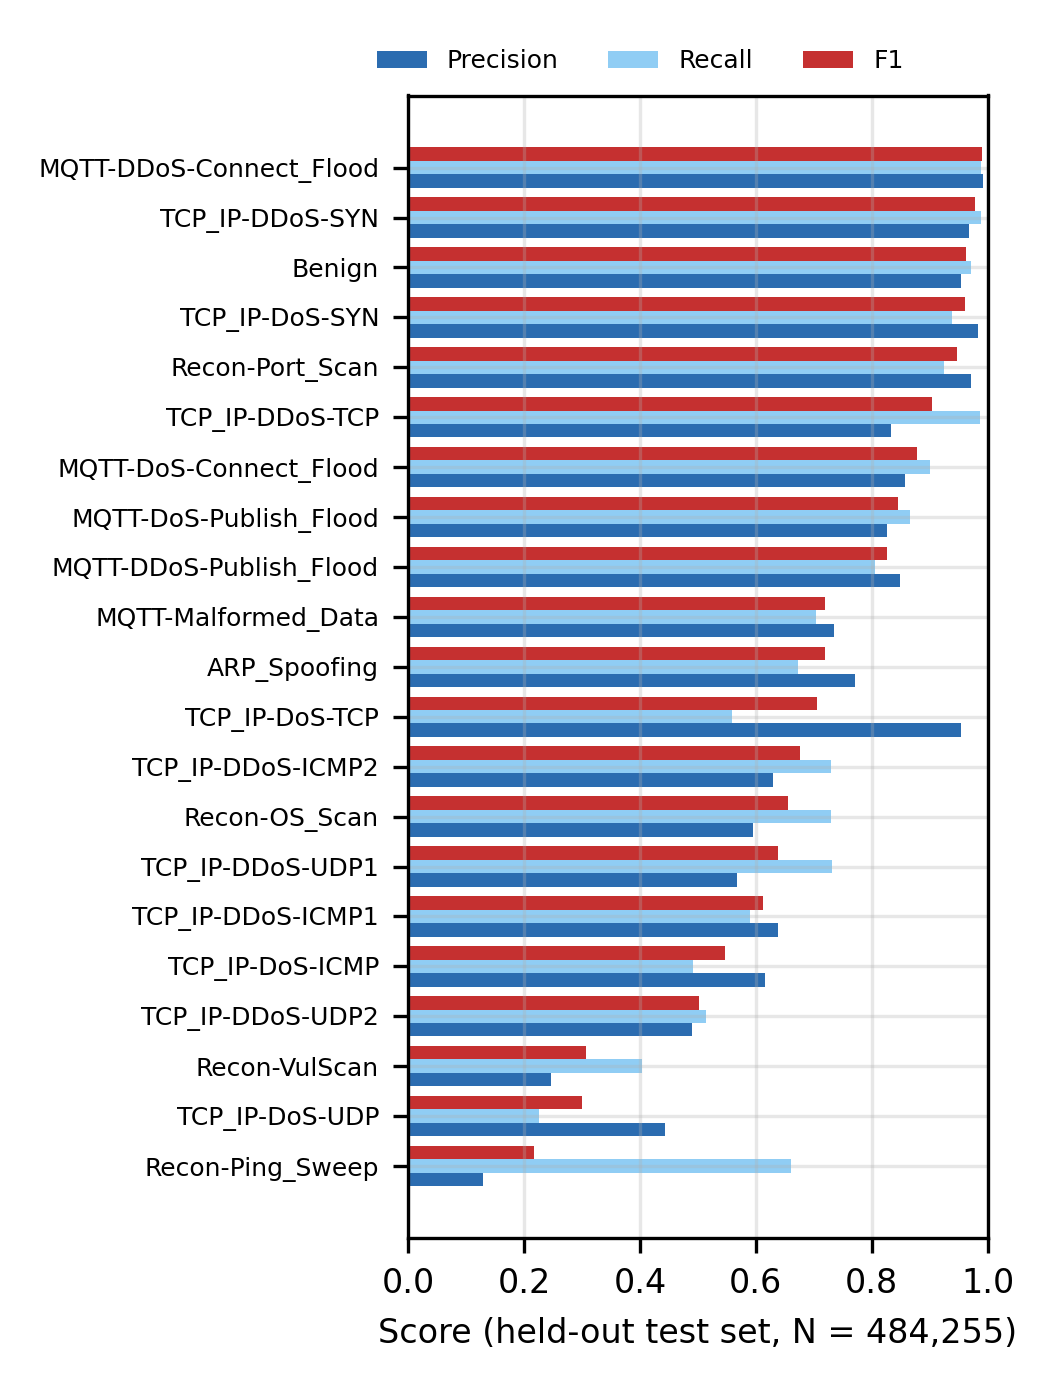
\includegraphics[width=\columnwidth]{fig_offline_per_class.png}
\caption{Per-class precision, recall, and F1 of the 21-class LightGBM model on the CICIoMT2024 held-out test set.}
\label{fig:offline}
\end{figure}

The standard deviation and minimum of the frame lengths account for 37.5\% of split gain, the five non-zero flag shares for 29.2\%, and packet rate for 8.2\% (Fig.~\ref{fig:fi}). Without the windowing and timing columns, the model separates traffic mainly by packet-size profile and TCP flag mix, which suits connection-oriented attacks and scans but not floods whose packets resemble benign telemetry.

\begin{figure}[!t]
\centering
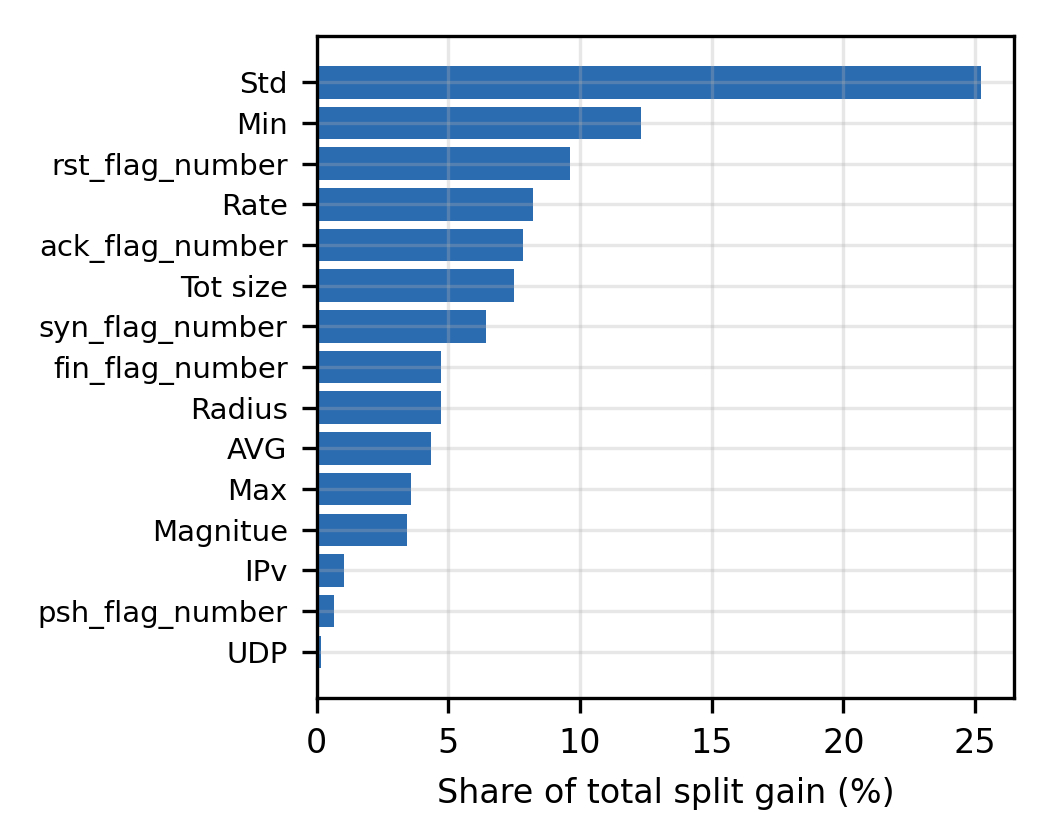
\includegraphics[width=\columnwidth]{fig_feature_importance.png}
\caption{Top-15 features by share of total LightGBM split gain.}
\label{fig:fi}
\end{figure}

\subsection{Labelled Live Detection}
\label{sec:res-labelled}

Table~\ref{tab:live-detect} reports per-source flag rates in IDS mode, with each source alone (R1 for benign traffic, R2 for attacks) and all sources together (R3), and, for R3, the flag rates of the model's raw predictions before the client-share rule.

\textit{Benign Only (R1):} 1.0$\pm$0.5\% of benign-client verdicts and none of the gateway-subscriber verdicts were attacks (accuracy 98.96$\pm$0.55\%), close to the offline benign error. Per connection the picture differs: every benign connection lasted the whole session and received 34--121 verdicts, so the mixed client drew at least one attack verdict in all four runs, the burst client in three, the monitoring subscriber in one, and the steady client and the gateway subscriber in none. No connection drew two consecutive attack verdicts, so the $K = 2$ policy would have blocked none of them, whereas blocking after a single verdict would have blocked 2.0$\pm$0.8 per session.

\textit{Attacks Alone (R2):} Per-verdict precision was 1.000, recall 0.994$\pm$0.001, and F1 0.997$\pm$0.001. Because R2 contains no benign clients, its precision cannot reveal false positives and does not describe mixed traffic. Every verdict on SYN-flood, slow-connection, port-scan, vulnerability-scan, and both UDP-flood connections was an attack, as were 99.4\% of the connect-flood verdicts (serial and parallel), all 232 publish-flood verdicts, and 91.9\% of the malformed-packet verdicts. The two UDP floods produce 2,880 of the 4,126 attack verdicts per session; without them, volume-weighted recall is 0.981. Macro-averaged recall over the ten attack families is 0.991$\pm$0.002 (0.988$\pm$0.003 without the two UDP families); the weakest family is malformed MQTT (0.919$\pm$0.009). The gateway subscriber, which in R2 received almost only forwarded attack messages, was flagged in 4.3\% of its verdicts (11 of 258 per session).

\textit{Combined (R3):} R3 is the relevant mixed-traffic result: per-verdict precision was 0.999$\pm$0.000, recall 0.994$\pm$0.001, F1 0.996$\pm$0.001, and accuracy 99.40$\pm$0.10\%; without UDP-flood verdicts, volume-weighted recall is 0.980 and accuracy 98.53$\pm$0.23\%. Macro-averaged recall over the ten families is 0.991$\pm$0.002 (0.989$\pm$0.002 without the two UDP families); again the weakest family is malformed MQTT (0.924$\pm$0.013). Attack flag rates matched R2 within one percentage point, the publishers were flagged in 1.7--4.2\% of their verdicts, the monitoring subscriber in none of its 564, and the gateway subscriber in 0.3\%. The client-share rule accounts for this: the model's raw predictions on the same verdicts flag 54.0\% of the monitoring subscriber's verdicts and 61.0\% of the gateway subscriber's, because the broker forwards the publish-flood and malformed payloads to both, and would give a precision of 0.930$\pm$0.003 and an accuracy of 93.3$\pm$0.3\%. The flow of a subscriber thus inherits the character of the traffic published to its topics; the rule removes this by crediting a prediction to the client only if the client sent the traffic, and it cost 0.2 percentage points of recall, mostly on connect floods and malformed packets.

\begin{table}[!t]
\centering
\caption{Live Detection by Traffic Source in IDS Mode. Flag Rate = Share of Verdicts Labelled Attack (\%, Mean $\pm$ SD Over Four Runs); Alone = R1 (Benign) or R2 (Attacks); Conn.\ and Verdicts From R3; Raw = Model Prediction in R3 Before the Client-Share Rule}
\label{tab:live-detect}
\footnotesize
\setlength{\tabcolsep}{3pt}
\resizebox{\columnwidth}{!}{%
\begin{tabular}{lrrrrr}
\toprule
 & & & \multicolumn{3}{c}{\textbf{Flag rate (\%)}} \\
\cmidrule(lr){4-6}
\textbf{Source} & \textbf{Conn.} & \textbf{Verdicts} & \textbf{Alone} & \textbf{Combined} & \textbf{Raw} \\
\midrule
Steady publisher        & 1     & 45.0    & 0.0$\pm$0.0   & 1.7$\pm$1.1 & 1.7 \\
Mixed publisher         & 1     & 60.2    & 3.4$\pm$2.3   & 4.2$\pm$1.7 & 4.2 \\
Burst publisher         & 1     & 54.8    & 1.7$\pm$1.2   & 1.8$\pm$1.5 & 1.8 \\
Monitoring subscriber   & 1     & 564.2   & 0.2$\pm$0.4   & 0.0$\pm$0.0 & 54.0 \\
Gateway subscriber (infra.) & 1 & 402.5   & 0.0$\pm$0.0   & 0.3$\pm$0.1 & 61.0 \\
\midrule
MQTT publish flood      & 1     & 232.5   & 100$\pm$0     & 99.9$\pm$0.2 & 99.9 \\
Malformed MQTT          & 1     & 237.0   & 91.9$\pm$0.9  & 92.4$\pm$1.3 & 92.7 \\
Slow connection (5 conn.) & 5   & 5.0     & 100$\pm$0     & 100$\pm$0   & 100 \\
MQTT connect flood      & 59.0  & 116.2   & 99.4$\pm$1.3  & 99.6$\pm$0.5 & 100 \\
MQTT connect flood (5 thr.) & 293.8 & 592.0 & 99.4$\pm$0.5 & 99.0$\pm$0.4 & 100 \\
Port scan               & 1     & 1.0     & 100$\pm$0     & 100$\pm$0   & 100 \\
Vulnerability scan      & 2     & 2.0     & 100$\pm$0     & 100$\pm$0   & 100 \\
UDP flood               & 1     & 1,402.0 & 100$\pm$0     & 100$\pm$0   & 100 \\
UDP flood (5 thr.)      & 5     & 1,473.0 & 100$\pm$0     & 100$\pm$0   & 100 \\
TCP SYN flood           & 60.0  & 60.0    & 100$\pm$0     & 100$\pm$0   & 100 \\
\midrule
\multicolumn{6}{l}{Benign-client flag rate, R1: 1.0$\pm$0.5\%} \\
\multicolumn{6}{l}{Precision / recall / F1, R2: 1.000 / 0.994$\pm$0.001 / 0.997$\pm$0.001} \\
\multicolumn{6}{l}{Precision / recall / F1, R3: 0.999$\pm$0.000 / 0.994$\pm$0.001 / 0.996$\pm$0.001} \\
\multicolumn{6}{l}{Recall without UDP-flood verdicts, R2 / R3: 0.981 / 0.980} \\
\multicolumn{6}{l}{Macro-averaged recall over 10 attack families, R2 / R3: 0.991$\pm$0.002 / 0.991$\pm$0.002} \\
\multicolumn{6}{l}{Precision, R3, raw model predictions: 0.930$\pm$0.003} \\
\bottomrule
\end{tabular}}
\end{table}

\subsection{Stage 1 Live Latency}
\label{sec:res-ids}

Table~\ref{tab:ids-latency} reports Stage~1 timing over the 50,026 verdicts of all 20 sessions. Median LightGBM inference takes 1.10~ms, and feature extraction plus inference plus decision 2.41~ms (P95 4.33~ms). Arrival of the triggering packet to verdict takes 2.86~ms (P95 5.14~ms) over the 46,088 inline-triggered verdicts; the 3,938 verdicts triggered by the idle reaper have no triggering packet and are excluded from this column. R1 verdicts are slower (median classification 3.76~ms) because benign verdicts are issued at 20 packets, whereas most connect-flood and SYN-flood verdicts fall at a few packets on FIN or RST. These values are processing costs, not detection delay. The time from the first packet of a classified segment to its verdict, which includes the millisecond-scale processing above, has a median of 0.19~s (P95 10.9~s), and every packet in that interval is admitted. In R2 and R3 the 20-packet segments of the UDP and publish floods close within tens of milliseconds, which lowers the median. The processing times are about three times the mean classification time (0.94~ms) that we measured in an earlier single-host session with the 45-feature model; the live runs did not record CPU frequency or throttling state, so we report them as measured.

\begin{table}[!t]
\centering
\caption{Stage~1 Live Timing per Verdict (Median, ms, Except Collect in s). Inspect = Arrival of the Triggering Packet to Verdict, Inline-Triggered Verdicts Only; Collect = First Packet of the Classified Flow Segment to Verdict, Including Classification Processing}
\label{tab:ids-latency}
\footnotesize
\setlength{\tabcolsep}{3pt}
\resizebox{\columnwidth}{!}{%
\begin{tabular}{lrrrrrr}
\toprule
\textbf{Run} & \textbf{Verdicts} & \textbf{Infer.} & \textbf{Classify} & \textbf{Inspect} & \textbf{Inspect P95} & \textbf{Collect} \\
\midrule
R1 & 1,453 & 1.488 & 3.761 & 4.497 & 5.771 & 6.060 \\
R2 & 17,535 & 1.079 & 2.345 & 2.753 & 4.790 & 0.119 \\
R3 & 20,990 & 1.068 & 2.332 & 2.734 & 4.853 & 0.191 \\
R4 & 5,036 & 1.229 & 2.768 & 3.472 & 5.592 & 3.327 \\
R5 & 5,012 & 1.151 & 2.528 & 3.143 & 5.524 & 3.263 \\
\midrule
\textbf{All} & \textbf{50,026} & \textbf{1.098} & \textbf{2.409} & \textbf{2.860} & \textbf{5.142} & \textbf{0.191} \\
\bottomrule
\end{tabular}}
\end{table}

\subsection{Inline Blocking}
\label{sec:res-e2e}

Tables~\ref{tab:ips-effect} and~\ref{tab:ips-block} compare the two IPS runs. Without blocking, every benign publish with return code 0 reached Stage~2 in all R1 and R3 runs, so any loss in R4 and R5 is caused by blocking. Detection and blocking are not interchangeable: a high per-verdict recall (Table~\ref{tab:live-detect}) does not mean that Stage~1 cut the connection off the broker.

\textit{Attack Suppression:} In both IPS runs every labelled attack connection received at least one verdict, so the connection-level detection rate was 100\%. The block rate was 80.6$\pm$1.2\% in R4 (340.3 of 422.3 connections) and 80.2$\pm$0.8\% in R5 (334.3 of 417.0). Table~\ref{tab:ips-block} splits that rate by family. Long-lived floods---publish, malformed MQTT, and both UDP floods---were blocked in every session (8 of 8 connections). Serial connect floods were blocked at 99.2\% (R4) and 97.3\% (R5), and the five-thread connect flood at 95.2\% in both runs. The remaining 82.0$\pm$5.0 (R4) and 82.8$\pm$3.3 (R5) connections received only one verdict and so never met $K = 2$. They fall into two groups.

\textit{Already closed:} About 77 of those 82 were SYN-flood attempts (all 60 in R4; 59.8 in R5), leftover connect-flood attempts (0.5 serial and 13.8 five-thread in R4; 1.5 and 13.5 in R5), and short scans (the port scan in most sessions and both vulnerability-scan connections). These attempts end within a few packets. A block after the classifying FIN or RST would cover only a finished tuple and would not have reduced broker state.

\textit{Still open:} All five slow-connection sockets were detected and none were blocked. Unlike the SYN and connect floods, they kept their broker sockets until the 60~s attack window ended, so the failure to block them left idle connections on the broker for the rest of the window. A two-verdict policy cannot cut off a connection that is classified only once, when it goes idle.

Up to and including the segment that triggered its block, a blocked attack connection carried 12.4 packets on average (median 12, both directions), all admitted. Afterwards, about 57,300 packets of blocked attack connections were dropped per session, most of them from the publish and UDP floods, and 466--518 packets that the broker sent to blocked connections were dropped as well. These drop counts reflect the attack rates of Section~\ref{sec:method} and are not comparable with sessions run at other rates. Flag rates in R4 and R5 match R3 except for the malformed-packet flow (65\%), which received only 3--4 verdicts before its block.

\textit{Collateral Blocking:} The gateway subscriber drew 0.5 and 0.8 attack verdicts per session in R4 and R5, never two in a row, so the allow-list of R4 never had to prevent a block, and no infrastructure connection was blocked in R5. One benign connection was blocked in one of the four sessions of each run (the mixed publisher, after 125~s in R4 and after 822~s in R5); its client reconnected on a new port, 12 of its packets were dropped in R4 and none in R5, and in every session all benign publishes with return code 0 reached Stage~2. Applied to the R3 verdicts, blocking after a single attack verdict would have blocked 2.5$\pm$0.6 benign and 1.0 gateway-subscriber connections per session, against 0 and 0.25 with $K = 2$, while blocking 427.5 rather than 346.0 attack connections. For comparison, the development sessions, which blocked after a single verdict, had no client-share rule, and ran their attacks at one event per second, blocked 13.0 (R4) and 8.3 (R5) benign connections per session, and delivered 88.6\% and 59.2\% of benign messages to Stage~2, the latter falling to 34--44\% in sessions in which the gateway subscriber itself was blocked. The two policies thus trade the blocking of single-verdict attack connections for the availability of long-lived benign connections and of Stage~2's own input.

\begin{table}[!t]
\centering
\caption{Effect of Inline Blocking (IPS Mode, $K = 2$, Mean $\pm$ SD Over Four Runs per Session)}
\label{tab:ips-effect}
\footnotesize
\setlength{\tabcolsep}{3pt}
\resizebox{\columnwidth}{!}{%
\begin{tabular}{lrr}
\toprule
\textbf{Metric} & \textbf{R4: allow-list} & \textbf{R5: no allow-list} \\
\midrule
Benign publishes (return code 0)       & 1,214.0$\pm$8.1   & 1,210.5$\pm$29.0 \\
Benign messages received by Stage~2    & 1,214.0$\pm$8.1   & 1,210.5$\pm$29.0 \\
Benign delivery ratio                  & 1.000$\pm$0.000   & 1.000$\pm$0.000 \\
\midrule
Attack connections                     & 422.3$\pm$3.2     & 417.0$\pm$6.3 \\
Attack connections blocked             & 340.3$\pm$6.3     & 334.3$\pm$6.1 \\
Attack-connection block rate           & 0.806$\pm$0.012   & 0.802$\pm$0.008 \\
Detected (any attack verdict)          & 1.000             & 1.000 \\
Detected, single verdict, not blocked  & 82.0$\pm$5.0      & 82.8$\pm$3.3 \\
\quad still on broker (slow conn.)     & 5.0$\pm$0.0       & 5.0$\pm$0.0 \\
\quad already closed (SYN, leftover connect, scans) & 77.0$\pm$5.0 & 77.8$\pm$3.3 \\
Attack connections never classified    & 0                 & 0 \\
Packets before block (per blocked attack conn.) & 12.38$\pm$0.07 & 12.31$\pm$0.06 \\
Attack packets dropped                 & 57,335$\pm$59     & 57,352$\pm$84 \\
Broker packets to blocked conn.\ dropped & 518$\pm$171     & 466$\pm$204 \\
\midrule
Benign-client packets dropped          & 3$\pm$6           & 0 \\
Infrastructure packets dropped         & 0                 & 0 \\
Benign connections blocked             & 0.25$\pm$0.50     & 0.25$\pm$0.50 \\
Infrastructure blocks prevented        & 0                 & -- \\
Infrastructure connections blocked     & 0                 & 0 \\
\bottomrule
\end{tabular}}
\end{table}

\begin{table}[!t]
\centering
\caption{Connection-Level Block Rate by Attack Family (IPS Mode, $K = 2$, Mean Over Four Runs). Detected = Share of Labelled Connections With at Least One Attack Verdict; Blocked = Share for Which a Block Was Applied. ``Held'' = the Broker Socket Was Still Open After the Miss}
\label{tab:ips-block}
\footnotesize
\setlength{\tabcolsep}{3pt}
\resizebox{\columnwidth}{!}{%
\begin{tabular}{lrrrr}
\toprule
\textbf{Family} & \textbf{Conns (R4)} & \textbf{Blocked R4} & \textbf{Blocked R5} & \textbf{Held?} \\
\midrule
MQTT publish flood           & 1      & 100\% & 100\% & -- \\
Malformed MQTT               & 1      & 100\% & 100\% & -- \\
UDP flood                    & 1      & 100\% & 100\% & -- \\
UDP flood (5 thr.)           & 5      & 100\% & 100\% & -- \\
MQTT connect flood           & 59.0   & 99.2\% & 97.3\% & no$^{\mathrm{a}}$ \\
MQTT connect flood (5 thr.)  & 287.3  & 95.2\% & 95.2\% & no$^{\mathrm{a}}$ \\
\midrule
TCP SYN flood                & 60.0   & 0\%   & 0\%   & no \\
Slow connection (5 conn.)    & 5      & 0\%   & 0\%   & yes \\
Port scan                    & 1      & 25\%  & 0\%   & no \\
Vulnerability scan           & 2      & 0\%   & 0\%   & no \\
\midrule
\textbf{All attack conn.}    & 422.3  & 80.6\% & 80.2\% & -- \\
\bottomrule
\multicolumn{5}{l}{\footnotesize $^{\mathrm{a}}$Unblocked leftovers only; blocked connect-flood sockets are cut off.} \\
\end{tabular}}
\end{table}

\subsection{Stage 2 Re-Encryption Cost}
\label{sec:res-pqc}

Table~\ref{tab:stage2} and Fig.~\ref{fig:stage2} report Stage~2 cost for the 18,157 messages received by the gateway subscriber in R1 and R3--R5 (187--214~B JSON payloads). The median re-encryption takes 2.073~ms: ML-DSA-65 signing dominates (1.413~ms), followed by ML-KEM-768 encapsulation (0.507~ms) and AES-GCM (0.110~ms). The full handler, including key derivation, MQTT dispatch, and JSON processing, has a median of 4.42~ms and a P99 of 9.48~ms. These values are about 13 times the median re-encryption time (0.156~ms) of an earlier single-host session in which clients, broker, and gateway shared one Pi; as for Stage~1, CPU frequency and thermal state were not recorded during the live runs. Even so, against publish intervals of seconds, the gateway-side cryptographic cost meets G5 by more than two orders of magnitude; G5 is not a measured end-to-end latency.

\begin{table}[!t]
\centering
\caption{Stage~2 Per-Message Gateway-Side Cost on Live Traffic (ms, $N = 18{,}157$ Messages Received by Stage~2 in R1 and R3--R5, Real liboqs)}
\label{tab:stage2}
\footnotesize
\setlength{\tabcolsep}{3pt}
\resizebox{\columnwidth}{!}{%
\begin{tabular}{lrrrrr}
\toprule
\textbf{Operation} & \textbf{Median} & \textbf{Mean} & \textbf{P95} & \textbf{P99} & \textbf{Max} \\
\midrule
ML-KEM-768 encap.     & 0.507 & 0.490 & 0.808 & 1.127 & 9.641 \\
AES-256-GCM encrypt   & 0.110 & 0.111 & 0.166 & 0.262 & 4.399 \\
ML-DSA-65 sign        & 1.413 & 1.651 & 3.669 & 5.420 & 25.372 \\
\midrule
Re-encryption total   & 2.073 & 2.252 & 4.508 & 6.294 & 25.874 \\
Full gateway handler  & 4.420 & 4.344 & 7.310 & 9.479 & 30.837 \\
\bottomrule
\end{tabular}}
\end{table}

\begin{figure}[!t]
\centering
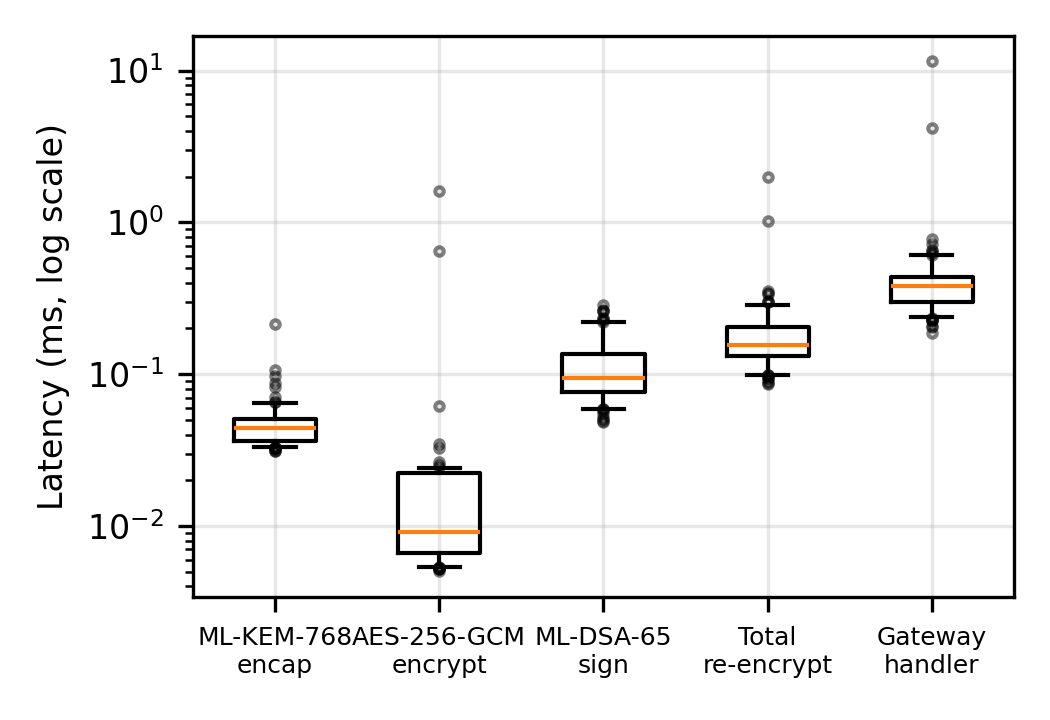
\includegraphics[width=\columnwidth]{fig_stage2_latency.png}
\caption{Distribution of Stage~2 per-message latency (box: interquartile range; whiskers: 5th--95th percentile).}
\label{fig:stage2}
\end{figure}

\textit{Bandwidth:} Re-encryption adds a fixed 4,425~B per message before encoding: the ML-KEM-768 ciphertext (1,088~B), the ML-DSA-65 signature (3,309~B), the nonce (12~B), and the GCM tag (16~B). This cost falls on the gateway-to-cloud uplink, not on the constrained device link.

\textit{Receiver Cost (Estimate):} A cloud receiver would perform the inverse operations: ML-KEM-768 decapsulation, AES-GCM decryption, and ML-DSA-65 verification. We do not measure a cloud receiver. As a reference, the gateway performs the same three operations in the separate scheme-comparison benchmark at a median of 0.772~ms per 5~KB message on the Raspberry Pi (Table~\ref{tab:matrix}), whereas live Stage~2 envelopes carried plaintext payloads of only about 200~B. This is a reference measurement, not a direct estimate of cloud latency; actual receiver cost depends on the cloud platform, software stack, and load, and excludes network transit.

\subsection{Choice of Post-Quantum Scheme}
\label{sec:res-matrix}

Table~\ref{tab:matrix} and Fig.~\ref{fig:matrix} compare ten configurations on the same gateway. Three tiers appear. In cryptographic time, ML-KEM pairings with ML-DSA or Falcon need 0.56--0.77~ms at 5~KB, about 36--53\% less than ECDH+ECDSA (1.21~ms), mainly because the measured ML-KEM decapsulation (0.13--0.19~ms) is 3--5$\times$ shorter than the P-256 ECDH timer (0.62~ms), whose boundary also includes point parsing and HKDF. The advantage depends on payload size: at 100~KB these pairings need 3.14--3.50~ms against 3.73~ms for ECDH+ECDSA. It also does not hold for total handler time (Table~\ref{tab:matrix}, Handler), where ECDH+ECDSA was faster at 5~KB (1.59~ms, against 1.85--2.32~ms for the ML-DSA pairings and 22.47~ms for ML-KEM-512 + Falcon-512) because its key objects were cached while the PQC key pairs were regenerated per message. SLH-DSA verification adds about 1~ms. FrodoKEM-640 (17.6~ms) and BIKE-L1 (36.1~ms) decapsulation dominate their pairings and produce the heaviest tails (P95 44--55~ms). At 100~KB, symmetric decryption grows to about 1.9~ms and narrows the gap: ML-KEM-768 + ML-DSA-65 costs 1.9$\times$ AES-only.

\begin{table*}[!t]
\centering
\caption{Gateway Receive Cost per Message (Median, ms) and Serialized MQTT Message Size. $L$ = Minimum NIST Level; $N = 600$ per Cell; Crypto = Decapsulation + Decryption + Verification Where Applicable; Handler = Total Gateway Handler Time, Including Per-Message PQC Key Regeneration (Classical Keys Cached)}
\label{tab:matrix}
\footnotesize
\begin{tabular}{lcrrrrrrrr}
\toprule
 & & \multicolumn{6}{c}{\textbf{5 KB payload}} & \multicolumn{2}{c}{\textbf{100 KB}} \\
\cmidrule(lr){3-8}\cmidrule(lr){9-10}
\textbf{Scheme (KEM + signature)} & \textbf{L} & \textbf{Decap} & \textbf{Verify} & \textbf{Crypto} & \textbf{P95} & \textbf{Handler} & \textbf{Msg. (B)} & \textbf{Crypto} & \textbf{Handler} \\
\midrule
ChaCha20-Poly1305          & -- & --     & --    & 0.073  & 0.143  & 0.403   & 7,327  & 0.424  & 2.371 \\
AES-256-GCM                & -- & --     & --    & 0.143  & 0.337  & 0.474   & 7,314  & 1.861  & 3.829 \\
ECDH + ECDSA P-256         & -- & 0.621  & 0.453 & 1.206  & 2.911  & 1.587   & 7,577  & 3.725  & 5.629 \\
\midrule
ML-KEM-512 + ML-DSA-44     & 1  & 0.130  & 0.260 & 0.562  & 1.514  & 1.852   & 11,604 & 3.283  & 6.177 \\
ML-KEM-512 + Falcon-512    & 1  & 0.129  & 0.279 & 0.572  & 1.456  & 22.472  & 9,253  & 3.140  & 25.954 \\
ML-KEM-768 + ML-DSA-65     & 3  & 0.194  & 0.433 & 0.772  & 2.125  & 2.321   & 13,216 & 3.497  & 6.603 \\
ML-KEM-768 + SLH-DSA-128s  & 1  & 0.167  & 1.363 & 1.723  & 2.317  & 156.515 & 19,293 & 4.458  & 161.630 \\
FrodoKEM-640 + ML-DSA-65   & 1  & 17.600 & 0.345 & 18.107 & 44.248 & 36.927  & 24,774 & 20.398 & 40.659 \\
FrodoKEM-640 + SLH-DSA-128s& 1  & 17.859 & 1.374 & 19.410 & 43.616 & 193.054 & 30,851 & 21.858 & 196.846 \\
BIKE-L1 + ML-DSA-44        & 1  & 36.126 & 0.248 & 36.550 & 54.794 & 81.711  & 12,677 & 39.093 & 85.673 \\
\bottomrule
\end{tabular}
\end{table*}

\begin{figure*}[!t]
\centering
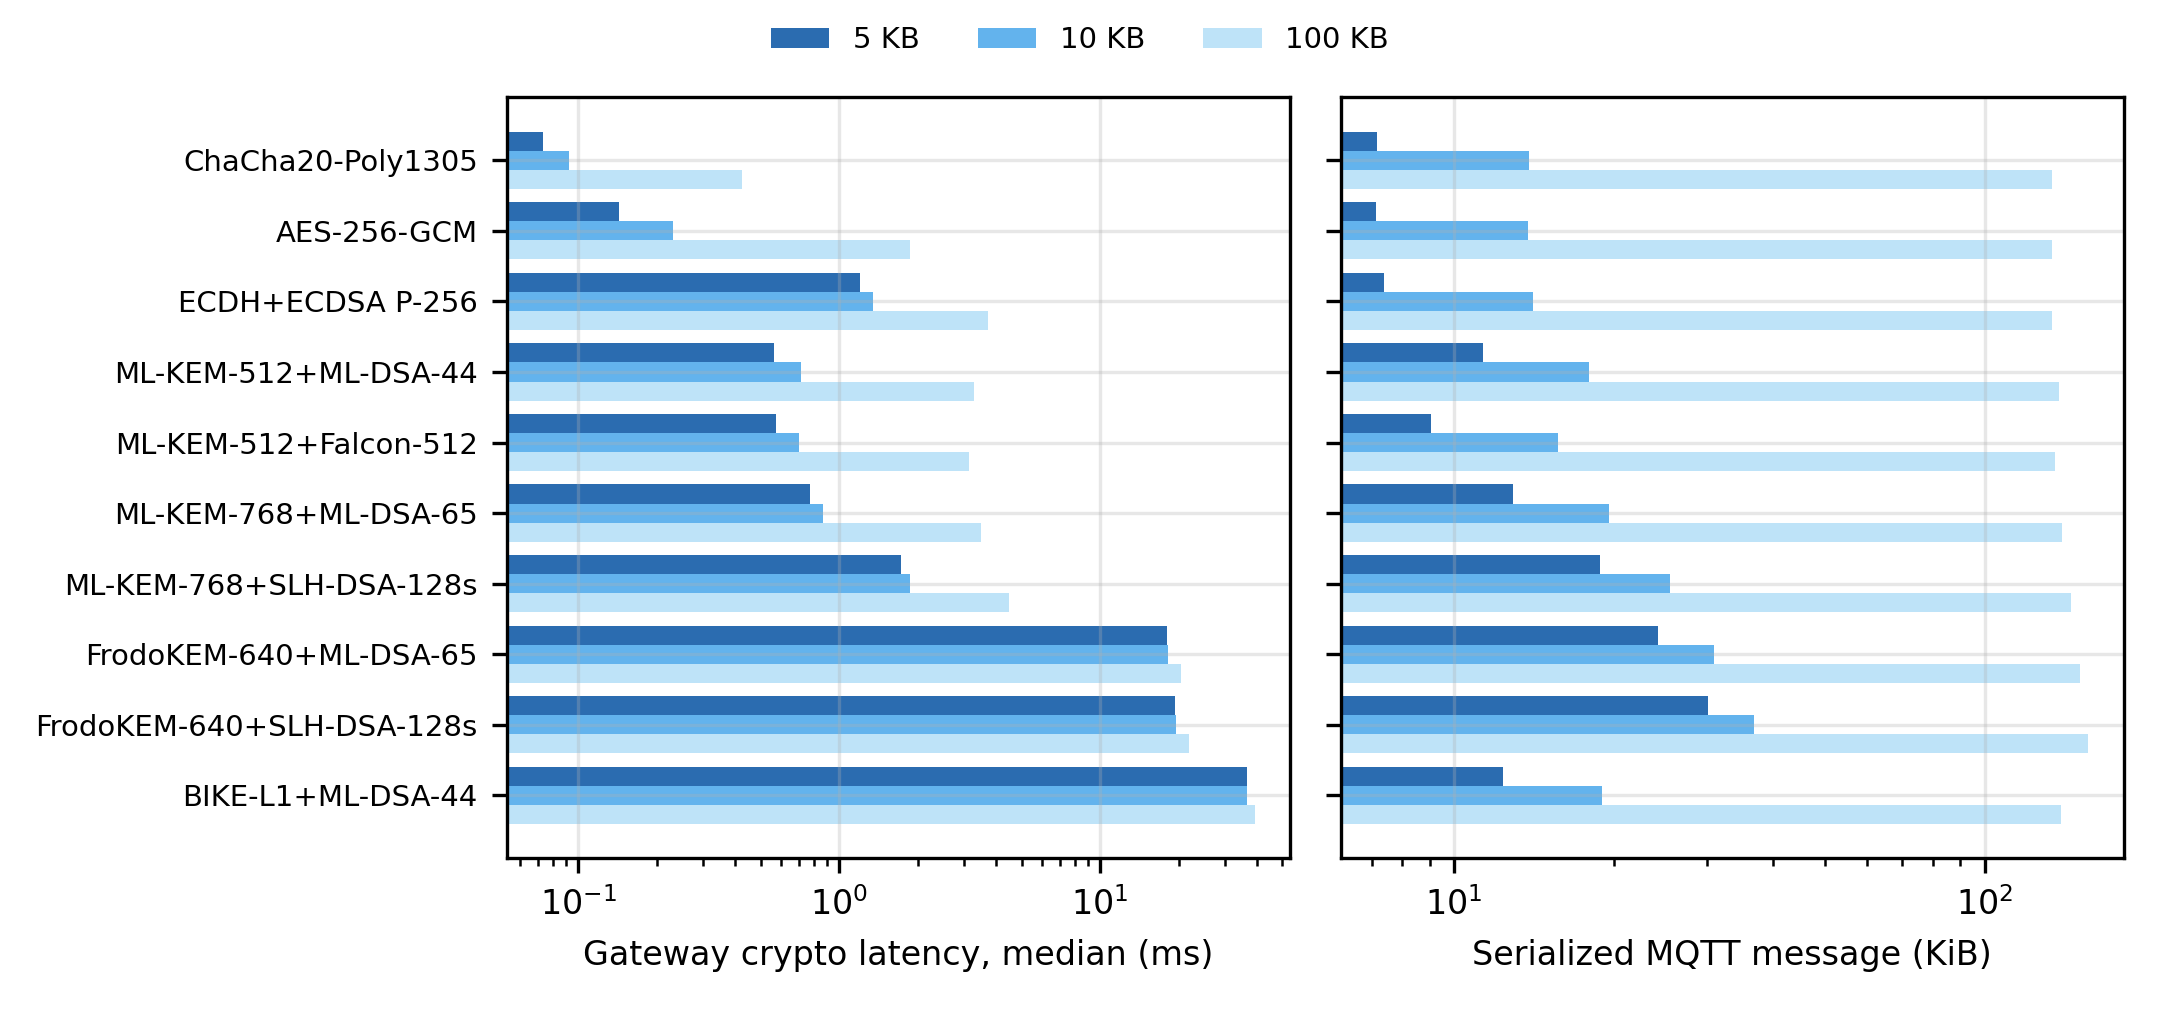
\includegraphics[width=0.9\textwidth]{fig_scheme_matrix.png}
\caption{Gateway cryptographic latency (left) and serialized message size (right) for ten configurations at three payload sizes (log scales).}
\label{fig:matrix}
\end{figure*}

\textit{Message Size:} Even AES-only expands a 5,120-byte payload to 7,314~B (+43\%) because of Base64 encoding and JSON metadata. Post-quantum material enlarges the 5~KB message by 1.27$\times$ (Falcon-512) to 4.22$\times$ (FrodoKEM + SLH-DSA) over AES-only, but only by 1.4--17\% at 100~KB, which favours batching small readings before protection.

\textit{Key Regeneration:} The PQC benchmark handler is stateless: it rederives the gateway KEM key pair and the device verification key for each message. The resulting non-cryptographic handler time, which includes key regeneration together with decoding, JSON handling, and logging, is 1.3--1.6~ms for ML-KEM/ML-DSA, 22~ms for Falcon-512, 19~ms for FrodoKEM, 45~ms for BIKE, and 155--174~ms for SLH-DSA, about 90$\times$ the cryptographic work. These figures are not pure key-generation latency: about 0.35~ms of non-cryptographic time is also observed in the AES-only, ChaCha20, and cached ECDH+ECDSA configurations. Practical gateways should cache keys per device and algorithm. Caching is expected to remove most of this overhead and to make Falcon and SLH-DSA viable, but a key-cached PQC handler was not measured.

\subsection{Three-Pi Testbed and Cloud Delivery}
\label{sec:res-three-pi}

Table~\ref{tab:three-pi} reports the follow-on campaign. It does not replace R1--R5. It asks whether the same Stage~1 policies still separate benign and attack traffic when benign publishers run on two addresses and attacks come from a second client, and whether a receiver accepts the Stage~2 envelope.

With both Pis publishing only benign traffic (E1, IPS), the benign flag rate was 3.0$\pm$0.7\% over eight long-lived client connections, no benign connection was blocked, and 0.997$\pm$0.001 of successful publishes reached Stage~2. There were no attack labels, so precision and recall are undefined. When Pi~B alone ran all ten attacks and Pi~A stayed benign, IDS mode (E2) gave precision 0.999, recall 0.991$\pm$0.000, and F1 0.995. The same split in IPS mode, on the two complete repetitions, gave precision 0.997$\pm$0.003, recall 0.976$\pm$0.001, and F1 0.986$\pm$0.002, with benign delivery 1.000 and no benign connection blocked. Splitting the attack list across the two Pis (E4 IDS, E5 IPS) gave F1 0.995$\pm$0.001 and 0.989$\pm$0.005. In E5 every successful benign publish reached Stage~2, and about 57,700 attack packets were dropped per session after a block, close to the two-Pi IPS runs. Pi~B completed all ten attacks in each E2 repetition.

The cloud receiver is not on the critical path of the MQTT callback. On the first dual-benign repetition it accepted 1,315 envelopes (902 from Pi~A, 413 from Pi~B). Median signature check, decapsulation, and decryption together took 0.209~ms. Attack-only traffic from Pi~B is not a Stage~2 publish, so later attack runs show cloud accepts only for Pi~A's benign publishers. Several later repetitions re-encrypted on the gateway but recorded no new cloud accepts, because the receiver was not continuously reachable or still held sequence state from an earlier process. Those repetitions are not used as cloud-delivery results. The receiver did reject replays when an old sequence number was posted again. This is LAN delivery of the constructed envelope, not a wide-area latency or an active attack on the uplink.

\begin{table}[!t]
\centering
\caption{Three-Pi Campaign (Mean $\pm$ SD). E1--E2 and E4--E5 use three repetitions; E3 uses two (one interrupted repetition excluded). Delivery is the share of benign publishes with return code 0 that reached Stage~2. Precision and recall are per verdict and are undefined for E1, which has no attacks.}
\label{tab:three-pi}
\footnotesize
\setlength{\tabcolsep}{3pt}
\resizebox{\columnwidth}{!}{%
\begin{tabular}{llrrr}
\toprule
\textbf{Run} & \textbf{Traffic} & \textbf{Prec.} & \textbf{Recall} & \textbf{Delivery} \\
\midrule
E1 (IPS) & Both Pis benign & -- & -- & 0.997$\pm$0.001 \\
E2 (IDS) & Pi~B, all attacks & 0.999 & 0.991 & -- \\
E3 (IPS) & Pi~B, all attacks & 0.997$\pm$0.003 & 0.976$\pm$0.001 & 1.000$\pm$0.000 \\
E4 (IDS) & Attacks split A/B & 1.000 & 0.991$\pm$0.002 & -- \\
E5 (IPS) & Attacks split A/B & 0.996$\pm$0.001 & 0.982$\pm$0.010 & 1.000$\pm$0.000 \\
\bottomrule
\end{tabular}}
\end{table}

% ═════════════════════════════════════════════════════════════════════════════
\section{Discussion}
\label{sec:discussion}

\subsection{Why the Two Stages Compose}

The stages address different adversaries at different layers, but simultaneous operation is not the same as experimentally validated end-to-end security or availability. Stage~1 acts in the packet path ahead of the broker, where attack connections can be cut off cheaply from flow statistics once classified, although client packets before the blocking verdict reach the broker (12.4 packets in both directions per blocked attack connection in our runs). Stage~2 acts on messages that the gateway subscriber receives, constructing a post-quantum envelope. The two-Pi study does not transmit it; the three-Pi study posts it over HTTPS (Section~\ref{sec:res-three-pi}). Stage~2 processes a message only while the gateway subscriber remains connected. The coupling between the stages is therefore not only the admitted traffic: a block of the gateway subscriber removes Stage~2's input altogether, as the development sessions without the client-share rule showed. Because the subscriber receives forwarded attack traffic, it is exactly the client that a flow classifier is most likely to misjudge. PQC work is therefore spent only on traffic that reaches Stage~2, not on packets that Stage~1 later drops, and long-term confidentiality of a transmitted envelope would not depend on the classifier being correct. The two stages also run as separate processes (packet callback vs.\ MQTT callback): Stage~1 inference can delay later packets waiting in the queue, but the Stage~1 and Stage~2 timers are not added to form an end-to-end latency.

\subsection{Deployment Guidance}

\begin{itemize}
  \item \textit{Scheme:} ML-KEM-768 + ML-DSA-65 uses NIST Level~3 parameter sets for under 0.8~ms of gateway cryptographic time at 5~KB, with the achieved security conditional on secure key generation and provisioning (Section~\ref{sec:keys}); its advantage over ECDH+ECDSA narrows with payload size, and PQC key caching would be needed for it to carry over to total handler time, which we have not measured; ML-KEM-512 + Falcon-512 is the most bandwidth-efficient Level~1 option; FrodoKEM and BIKE suit only latency-tolerant links.
  \item \textit{Keys:} Cache key pairs per device and algorithm; per-message derivation dominates cost for Falcon and SLH-DSA.
  \item \textit{Bandwidth:} The fixed PQC overhead is large for small messages; batch readings where latency allows.
  \item \textit{Features and Calibration:} Use only features that the live extractor can reproduce exactly, and calibrate on local benign traffic. Without either measure, the 45-feature model labelled 96\% of benign verdicts as attacks in our pilot; we did not separate the contribution of each measure.
  \item \textit{Direction:} Credit an attack prediction to a client only if the client sent the traffic. Subscribers inherit the character of the messages that they receive; without the client-share rule, 54--61\% of the subscribers' verdicts in mixed traffic were attacks.
  \item \textit{IPS Policy:} Block only after repeated attack verdicts, exempt infrastructure clients (the gateway's own subscriber and monitoring clients) as a further safeguard, start in IDS mode, and calibrate on local benign traffic before enabling blocking. Blocking after a single verdict cuts off a long-lived benign connection at its first false verdict, so a low per-verdict false-positive rate does not keep such connections unblocked. Requiring two consecutive verdicts kept benign delivery at 100\% and blocked 81\% of attack connections, including every long-lived flood. The 19\% not blocked had been detected: SYN-flood and leftover connect-flood attempts had typically already closed, so a late block would not have cut a live socket, whereas all five slow-connection sockets remained open on the broker. Short floods need a per-host or rate-based control; slow connections need a policy that can act on a single idle verdict or on hold time.
\end{itemize}

\subsection{Limitations}
\label{sec:limits}

\begin{itemize}
  \item \textit{Testbed:} The two-Pi study uses one client address. The three-Pi study adds a second client address for benign load and for attacks, including a split of the attack list, but it is still three Pis on one Wi-Fi LAN, not a many-device deployment.
  \item \textit{Attack Coverage:} Eight of the ten generators still send one event per second per thread. The publish flood was raised to about 80 packets/s, within the dataset median, and the UDP floods to 500 packets/s with 50-byte frames, well below the dataset medians of about 21,000--27,000 packets/s. ICMP floods and replay were excluded. An attacker who makes the broker send it most of the payload bytes, for example by subscribing to many topics, can push its own share below $\gamma$ and evade the client-share rule.
  \item \textit{Ground Truth:} Labels come from client-side logs and attack time windows, not from per-packet tags; flows near window boundaries can be mislabelled. Every classified client-Pi flow of the reported sessions received a label.
  \item \textit{Calibration:} The model was calibrated on a pilot session that used the same benign generators and gateway subscriber as the evaluation, so the live false-positive rates are optimistic for unseen benign devices. Feature restriction and calibration were introduced together, and their individual effects were not measured. The 32-feature model also loses offline accuracy (71.5\% vs 97.85\%) relative to the 45-feature model.
  \item \textit{Offline Split:} Training and test rows come from one released dataset partition and are split by row, not by capture, so the offline metrics may be optimistic relative to unseen captures.
  \item \textit{Detection Metrics:} Precision, recall, and F1 are per verdict; they weight sources by verdict count, so in IDS sessions recall is dominated by the UDP floods (about 2,880 of 4,120 attack verdicts). We also report recall without those verdicts, the flag rate of every attack family, a macro-averaged recall over the ten families, and connection-level block rates (Table~\ref{tab:ips-block}). A detected connection is not necessarily a blocked one.
  \item \textit{Timing Conditions:} The live Stage~1 and Stage~2 timings are about 3 and 12 times higher than in an earlier single-host session; CPU frequency, governor, and throttling state were not recorded, and the cause is not established.
  \item \textit{Enforcement Delay:} We measure packets admitted before a verdict and packets dropped afterwards, but not the time from a verdict to the first enforced drop.
  \item \textit{Evasion:} An adversary who knows the features can shape traffic to look benign; adversarial robustness is not evaluated.
  \item \textit{Scheme Benchmark:} Configurations ran sequentially without independent repetitions, timer boundaries are implementation-specific (Section~\ref{sec:method}), and the PQC and classical handlers use different key-caching policies.
  \item \textit{Runtime:} All components run in Python, which adds dispatch and parsing overhead; no native implementation was measured, so we cannot quantify how the reported latencies would change.
  \item \textit{Joint Evaluation:} R1--R5 measure benign delivery to Stage~2, not to a cloud receiver. The three-Pi study posts envelopes over HTTPS and records accepts, duplicates, and replays on a LAN receiver. That does not include an HNDL observer or an active forgery of the uplink (G2, G3).
  \item \textit{Cloud Receiver:} The receiver is a PC on the same LAN, not a wide-area cloud. Several later repetitions re-encrypted on the gateway but recorded no new accepts. WAN latency is not measured. The 0.772~ms gateway receive-side reference in Section~\ref{sec:res-pqc} is separate from the 0.209~ms median measured on the receiver for the first dual-benign repetition.
  \item \textit{Not Measured:} End-to-end message latency including WAN transit, energy, and multi-gateway scaling. One E3 repetition was interrupted and is excluded from Table~\ref{tab:three-pi}.
  \item \textit{Key Management:} All keys derive from one shared master secret under the trust assumptions of Section~\ref{sec:keys}; this is a testbed convenience and a single point of failure, not a production provisioning scheme. The live sessions generate PQC key pairs from a non-repeating SHAKE-256 stream keyed by that secret; the scheme comparison used an earlier cyclic 64-byte seed. Neither construction is a cryptographically secure, independently provisioned generator, so the experiments do not establish production-grade post-quantum security.
\end{itemize}

% ═════════════════════════════════════════════════════════════════════════════
\section{Conclusion}
\label{sec:conclusion}

We presented a two-stage MQTT gateway that classifies live MQTT-bound flows with a LightGBM model in the kernel packet path, blocks a client connection after two consecutive attack verdicts, and constructs an ML-KEM-768 + AES-256-GCM + ML-DSA-65 envelope on messages that reach Stage~2. The primary evaluation is a labelled two-Pi testbed (five run types, four repetitions each, after separate development trials). A follow-on three-Pi campaign places benign publishers on two client addresses and attacks on one or both, and posts the envelope over HTTPS to a LAN receiver. A pilot with a model that used all 45 dataset features flagged 96\% of benign verdicts. After the model was restricted to features that a live flow can reproduce and calibrated on that pilot's benign traffic (two changes whose individual effects we did not separate), and after a client-share rule and a two-verdict blocking policy were set on development sessions, benign-only runs flagged 1.0\% of verdicts. In mixed traffic, per-verdict precision was 0.999 and recall 0.994 (0.980 without UDP-flood verdicts; macro-averaged recall over the ten attack families 0.991); every attack family, including the publish and UDP floods, was flagged in at least 91\% of its verdicts. The model's raw predictions on the same mixed-traffic verdicts give a precision of only 0.930, because subscribers receive forwarded attack traffic. Stage~1 needs a median 2.4~ms of processing per verdict and Stage~2 a median 2.1~ms of cryptographic work per message; these are separate gateway costs, not a measured end-to-end latency. Inline blocking cut off 81\% of attack connections after about 12 packets and delivered every benign message to Stage~2, with and without an allow-list for the gateway's own clients. Long-lived floods were always blocked. The 19\% not blocked had been detected on a single verdict: SYN-flood and leftover connect-flood attempts had typically already closed, whereas all five slow-connection sockets stayed open on the broker. On the three-Pi testbed the same policies kept benign delivery at 0.997 with two benign clients and at 1.000 when a second client attacked (E3, two repetitions; E5, three). IDS and IPS F1 stayed at 0.986--0.995. The LAN receiver accepted 1,315 envelopes in the first dual-benign repetition (median verify-and-decrypt 0.209~ms), including traffic from both clients; later repetitions were not uniformly logged at the receiver. Across ten configurations, ML-KEM pairings with ML-DSA or Falcon needed less cryptographic time than ECDH+ECDSA at 5~KB, an advantage that narrows at 100~KB and that the per-message PQC key regeneration outweighed in total handler time; key caching is therefore expected, though not yet measured, to decide both this comparison and whether Falcon and SLH-DSA are practical. Future work will evaluate per-host controls for short attacks, UDP floods at dataset rates, independently provisioned device keys, energy, many-device deployments, wide-area cloud latency, adversarially robust detection, and a native implementation.

\bibliographystyle{IEEEtran}
\bibliography{bib/references_journal}

\end{document}
